\documentclass[twocolumn,10pt,a4j]{jsarticle}
\usepackage{kougai}
\usepackage{dcolumn}

\title{主体性を養う反転授業の提案}
\author{1632024 植本 匠海  指導教員 須田 宇宙 准教授}
\date{}

\begin{document}

\maketitle

\section{はじめに}
近年では時代の変化がとても早い中で,主体性を持ち自ら学び,考え,行動できる人材が必要とされている.しかし,教育の場で受動的な学習が行われている原因の1つとして主体性が低いことが挙げられる.また,主体性を向上させる新しい学習方法として自宅などで基礎知識を学んだあとに課題や応用を授業時間内に行う反転授業が注目されている.

しかし,三田\cite{mita}の研究では予習動画をすべて見た学生が3割以下であることや,大谷ら\cite{ootani}のグループ学習を取り入れた研究では学生ごとの主体性の違いが原因で主体性が高い学習者のみで進めてしまい,その他の学習者が積極的に参加しなくても授業が進んでしまっていることなど,学習者それぞれの主体性の違いが問題点として報告されている.

そこで本研究では反転授業のグループ学習において,主体性を高めるために各々の学生を責任ある立場に付かせてグループワークを行ってもらう.授業終了後にアンケート調査を行い学生の主体性の違いを分析することを目的とする.

\section{実験の構想}
本研究では2019年後期に開講される情報数学応用の履修者を対象に対照実験を行う.授業の内容は自宅などでの事前学習でパスワードのハッシュ化について学び,授業時間内に事前学習の内容を踏まえて実際にGoogle Colaboratory上でプログラムを作成してもらうというものである.

責任者決めないクラスをA群として従来通りの反転授業のグループ学習を行ってもらう.責任者決めるクラスはB群としてグループで課題作成を行うときに課題作成の進捗項目を構想,プログラミング,検証の三種類に分けた.その流れを図1に示す.それぞれの進捗に合わせた責任者を決めその責任者を中心に作業を行い課題を完成させる.\newline


\begin{figure}[h]
\begin{center}
\scalebox{0.75}[0.75]{
 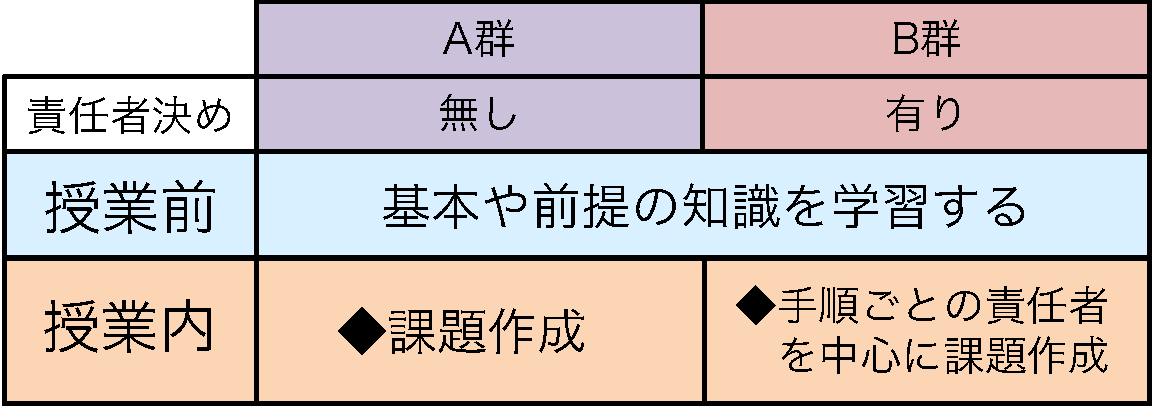
\includegraphics[clip,width=85mm,height=40mm]{nagare12.pdf}
 }
\end{center}
 \caption{責任者決め有り,無しの学習の流れ}
 \label{fig:流れ}
\end{figure}

授業の最後にそれぞれの群で主体性の違いを測るためのアンケートを行う.アンケートの内容は事前学習や課題作成にしっかりと取り組むことができたか,意見を出せたかなど主体性について尋ねた.これに加えてB群は責任者として率先して行動できたかを尋ねた.


\section{結果と考察}
各クラスのアンケートの5段階(1:できなかった〜5:できた)の内,4と5を合計した結果の一部を表1に示す.
表1より「主体的に取り組むことができたか」という質問に対してA群に比べてB群の方が僅かに増加したが,他の質問では低下した.

この原因として事前動画の視聴率の低さが挙げられる.アンケートによるとA群に比べてB群は事前学習用動画を見ている学生が少なかったため上昇しなかったと考えられる.
また,動画を視聴した学生は多いが,授業開始前までの視聴回数は少なく,何度も視聴している学生もいるとすると全体の6割程度しか視聴していない可能性がある.本研究では一部の学生が反転授業として今回の作成課題に取り組めていなかったと思われる.

他にも作業時間が少なかったため担当になった作業の意見を考えることで時間が取られてしまい意見を出したりグループワークに参加できなかったことも結果から推測される.

これらのことから改善点として一度だけではなく数回の反転授業を行い学生に慣れさせる必要があったと考えられる.また,作業時間を増やすなどグループ学習に向いた教室で行うことやiPadでの開発や慣れた言語で開発を行う必要もあったなどが挙げられた.\newline

\begin{table}[!hbt]
\begin{center}
\caption{アンケート結果(一部)}
\label{my-label}
\scalebox{0.85}[0.85]{
\begin{tabular}{|c|c|c|}
\cline{1-3}
 質問内容 & クラスA & クラスB \\ \cline{1-3}  
主体的に取り組むことができたか & 60.9 & 61.6 \\ \cline{1-3}  
 意見を出すことができたか & 60.9 & 57.7 \\ \cline{1-3}  
グループ全員が参加できていたか & 58.7 & 48.1 \\ \cline{1-3}  
普段の授業に比べて主体的に取り組めたか & 52.2 & 48.1 \\ \cline{1-3}  

\end{tabular}
}
\end{center}
\end{table}

\section{終わりに}
本研究では反転型授業のグループ学習において作業工程ごとの責任者を決めるという新たな手法を取り入れることで学生の主体性の養うことを目的とした実験を行った.今回の実験では実証することができなかったが,改善点が見つかったため,今後さらなる研究が望まれる.
\begin{thebibliography}{99}
\bibitem{mita} 三田満男「反転授業の実践とその課題」日本医療科学大学,日本科学教育研究会研究報告,Vol.31,No.5,(2017),2019/8/25参照
\bibitem{ootani} 大谷千恵,田村恵理子,河野功幸,根津幸徳,池田敦 「文系授業における反転授業の事例研究」玉川大学教育学部紀要 第17号 2017, pp117~142,2019/10/25参照
\end{thebibliography}


\end{document}